% figures/ragged-softmax-phases.tex
% Stable ragged softmax: one CTA per segment, three block-stride
% passes synchronized and broadcast by uniform gpu.all_reduce.
\documentclass[tikz,border=10pt]{standalone}
% figures/common-preamble.tex
% Shared setup for the TikZ documentation figures. Colors mirror the
% palette in scripts/render_docs_diagrams.py so both atlases match.
\usepackage[T1]{fontenc}
\usepackage{lmodern}
\usepackage{tikz}
\usepackage{pgfplots}
\pgfplotsset{compat=1.18}
\usetikzlibrary{arrows.meta}
\usetikzlibrary{backgrounds}
\usetikzlibrary{calc}
\usetikzlibrary{decorations.pathreplacing}
\usetikzlibrary{fit}
\usetikzlibrary{positioning}

\definecolor{swcanvas}{HTML}{FFFDF8}
\definecolor{swpanel}{HTML}{F5F3ED}
\definecolor{swink}{HTML}{17212B}
\definecolor{swmuted}{HTML}{4B5563}
\definecolor{swline}{HTML}{59636E}
\definecolor{swblue}{HTML}{00689D}
\definecolor{swbluefill}{HTML}{DCEFFD}
\definecolor{swpurple}{HTML}{8E4775}
\definecolor{swpurplefill}{HTML}{F7E2EF}
\definecolor{sworange}{HTML}{A94500}
\definecolor{sworangefill}{HTML}{FCE5DC}
\definecolor{swgreen}{HTML}{00664B}
\definecolor{swgreenfill}{HTML}{DDF4EB}
\definecolor{swgrayfill}{HTML}{EEF0F2}

\pagecolor{swcanvas}
\AtBeginDocument{\color{swink}}

\tikzset{
  swcell/.style={
    draw, minimum width=0.46cm, minimum height=0.46cm, inner sep=0pt,
    line width=0.7pt, rounded corners=1pt},
  swbox/.style={
    draw=swline, fill=swpanel, rounded corners=6pt, line width=0.9pt},
  swarrow/.style={-{Stealth[length=6pt]}, draw=swline, line width=1pt},
  swtag/.style={
    draw, rounded corners=8pt, line width=0.9pt,
    font=\bfseries\scriptsize, inner xsep=8pt, inner ysep=4pt},
  swtitle/.style={anchor=west, font=\Large\bfseries, text=swink},
  swsubtitle/.style={anchor=west, font=\small, text=swmuted},
  swcode/.style={font=\small\ttfamily, text=swink},
  every picture/.style={line cap=round},
}

\begin{document}
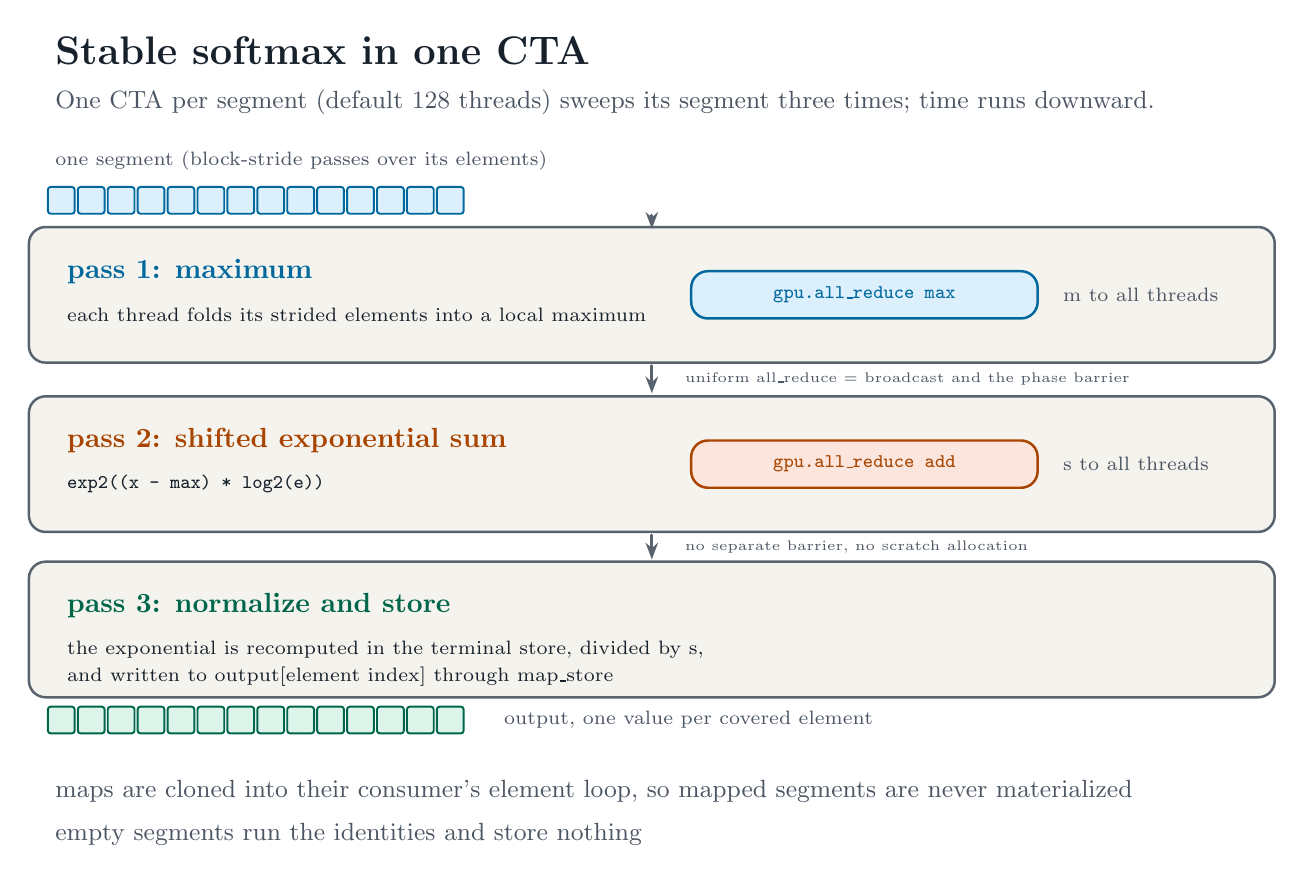
\begin{tikzpicture}[x=1cm, y=1cm]

% Header.
\node[swtitle] at (0, 1.15) {Stable softmax in one CTA};
\node[swsubtitle] at (0, 0.5)
  {One CTA per segment (default 128 threads) sweeps its segment three
   times; time runs downward.};

% The segment the CTA owns.
\node[anchor=west, font=\scriptsize, text=swmuted] at (0, -0.25)
  {one segment (block-stride passes over its elements)};
\foreach \i in {0,...,13} {
  \node[swcell, minimum width=0.34cm, minimum height=0.34cm,
        fill=swbluefill, draw=swblue] at ({0.2 + \i * 0.38}, -0.75) {};
}

% Phase 1: maximum.
\node[swbox, fit={(0, -2.6) (15.4, -1.3)}, inner sep=6pt] {};
\node[anchor=west, font=\bfseries, text=swblue] at (0.15, -1.65)
  {pass 1: maximum};
\node[anchor=west, font=\scriptsize, text=swink] at (0.15, -2.2)
  {each thread folds its strided elements into a local maximum};
\node[swbox, draw=swblue, fill=swbluefill, minimum width=4.4cm,
      minimum height=0.6cm] at (10.4, -1.95) {};
\node[font=\scriptsize\ttfamily, text=swblue] at (10.4, -1.95)
  {gpu.all\_reduce max};
\node[anchor=west, font=\scriptsize, text=swmuted] at (12.8, -1.95)
  {m to all threads};

% Phase 2: shifted exponential sum.
\node[swbox, fit={(0, -4.75) (15.4, -3.45)}, inner sep=6pt] {};
\node[anchor=west, font=\bfseries, text=sworange] at (0.15, -3.8)
  {pass 2: shifted exponential sum};
\node[anchor=west, font=\scriptsize\ttfamily, text=swink]
  at (0.15, -4.35) {\detokenize{exp2((x - max) * log2(e))}};
\node[swbox, draw=sworange, fill=sworangefill, minimum width=4.4cm,
      minimum height=0.6cm] at (10.4, -4.1) {};
\node[font=\scriptsize\ttfamily, text=sworange] at (10.4, -4.1)
  {gpu.all\_reduce add};
\node[anchor=west, font=\scriptsize, text=swmuted] at (12.8, -4.1)
  {s to all threads};

% Phase 3: normalize and store.
\node[swbox, fit={(0, -6.85) (15.4, -5.55)}, inner sep=6pt] {};
\node[anchor=west, font=\bfseries, text=swgreen] at (0.15, -5.9)
  {pass 3: normalize and store};
\node[anchor=west, font=\scriptsize, text=swink] at (0.15, -6.45)
  {the exponential is recomputed in the terminal store, divided by s,};
\node[anchor=west, font=\scriptsize, text=swink] at (0.15, -6.8)
  {and written to output[element index] through map\_store};

% Phase separators: the all_reduce is the barrier.
\draw[swarrow] (7.7, -0.94) -- (7.7, -1.11);
\draw[swarrow] (7.7, -2.85) -- (7.7, -3.2);
\node[anchor=west, font=\tiny, text=swmuted] at (8.0, -3.02)
  {uniform all\_reduce = broadcast and the phase barrier};
\draw[swarrow] (7.7, -5.0) -- (7.7, -5.31);
\node[anchor=west, font=\tiny, text=swmuted] at (8.0, -5.15)
  {no separate barrier, no scratch allocation};

% Output row.
\foreach \i in {0,...,13} {
  \node[swcell, minimum width=0.34cm, minimum height=0.34cm,
        fill=swgreenfill, draw=swgreen] at ({0.2 + \i * 0.38}, -7.35) {};
}
\node[anchor=west, font=\scriptsize, text=swmuted] at (5.7, -7.35)
  {output, one value per covered element};

% Fusion and edge-case notes.
\node[anchor=west, font=\small, text=swmuted] at (0, -8.25)
  {maps are cloned into their consumer's element loop,
   so mapped segments are never materialized};
\node[anchor=west, font=\small, text=swmuted] at (0, -8.8)
  {empty segments run the identities and store nothing};

\end{tikzpicture}
\end{document}
